\subsection{Conclusions}
The total uncertainty of the hygrometer measurement obtained after including the calibration error, repeatability and the hysteresis is $1.7$\% RH. For the array sensors, the uncertainty is about $4\%$.


As the hygrometer design turned out to be more consistent and robust, its performance was also compared with the E20 sampling system~\cite{michell_e20} and its ceramic sensor. The array did not provide the expected repeatability, and it  will be further tested inside the thermal demonstrator (see section~\ref{demo}). Moreover, below \SI{-20}{\celsius} the attenuation of the signals was observed, which may be related to the design of the packaging of the array sensors.

The performance of the hygrometer was confirmed during the low-temperature tests with the industrial capacitive sensors and the trace humidity sensor, what is summarized in Figure~\ref{fig_comparison}. The uncertainties of the sensors are not shown, in order to highlight the trends of the respective sensors. The largest uncertainty is associated with the SHT85 capacitive sensor. The ceramic sensor dew-point values are characterized by low uncertainty of up to \SI{1}{\celsius}.  
\begin{figure}[!h]
\centering
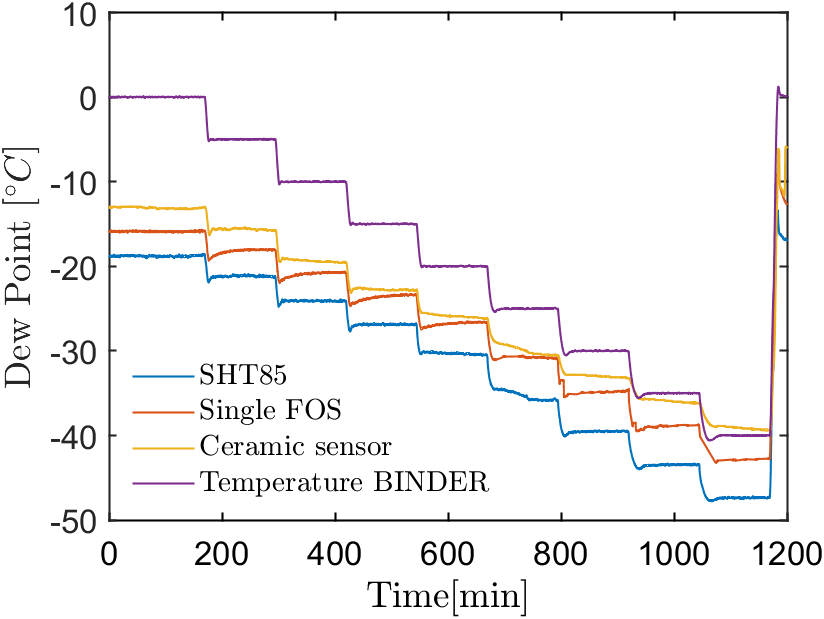
\includegraphics[width=0.6\columnwidth]{Chapter5/images/DPCPercent.png}
\caption{Comparison of the dew points calculated using the Magnus formula for the industrial sensor SHT85, metal oxide trace humidity sensor (ceramic sensor), and the hygrometer. For the comparison, the temperature inside the Binder climatic chamber was also plotted.}
\label{fig_comparison}
\end{figure}

The response of the hygrometer was also compared with the sampling system and different lengths of the guidelines leading to the ceramic sensor. In the final detector, the sampling system electronic circuitry will be placed at least \SI{20}{\metre} away from the detector. The tubing is going to increase the response time of the sampling system. 

Figure~\ref{fig_comparison_hw} shows the comparison of the results obtained with two different lengths of leading tubes. The tube length was \SI{2}{\metre} and \SI{12}{\metre}, for the left and right figure, respectively. The obtained time response was 1.5\,min and 3\,min. Assuming that the flow does not depend on the distance from the sampling point if the tube was \SI{30}{\metre} the response would be 5.7\,min. 
\begin{figure}[!h]
\centering
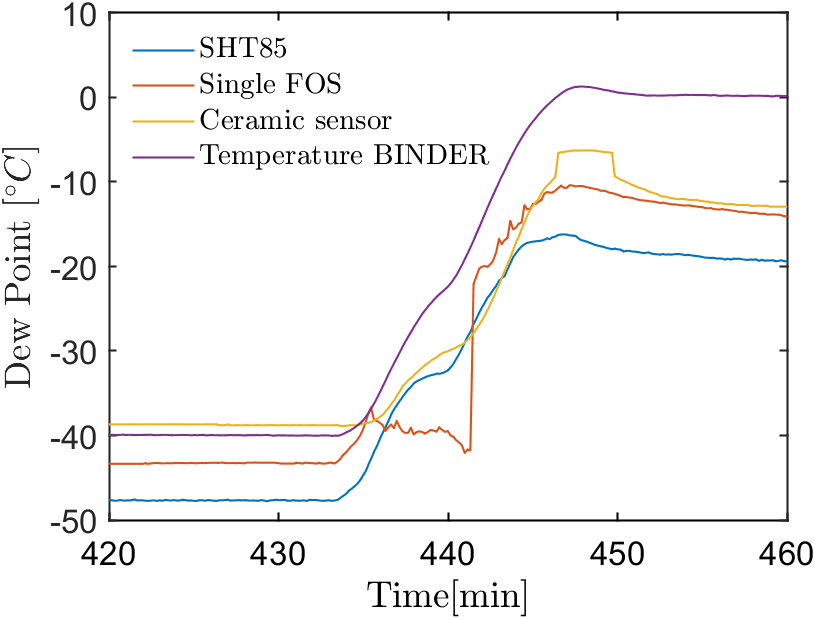
\includegraphics[width=0.47\columnwidth]{Chapter5/images/DPCPercent_response2m.png}
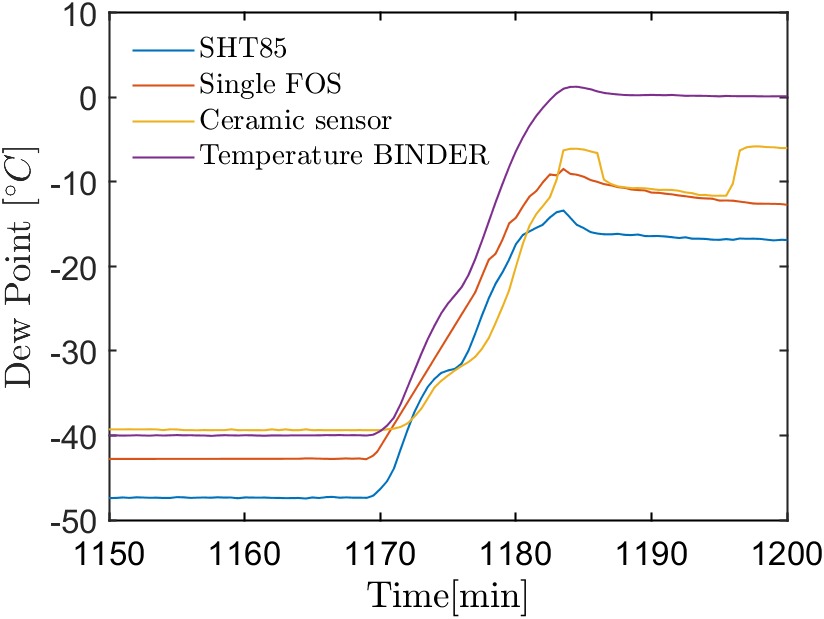
\includegraphics[width=0.47\columnwidth]{Chapter5/images/DPCPercent_response12m.png}
\caption{Time response comparison of different sensors. Left - \SI{2}{\metre} tube to the ceramic sensor, right - \SI{12}{\metre} tube to the ceramic sensor.}
\label{fig_comparison_hw}
\end{figure}
\newpage
Figure \ref{Tfig_comparison_2} shows the behavior of the \gls{FBG}-based hygrometer at low dew points. The sensing limits are clearly represented in Figure~\ref{Tfig_comparison_2}. The hygrometer performance is limited to the dew point of \SI{-70}{\celsius} (see the area highlighted with the red rectangle). Nevertheless, at such low dew points, the uncertainties become much higher. It is also noteworthy that that limit refers to the ambient temperature of \SI{10}{\celsius}. On the other hand, for the measurements at \SI{20}{\celsius} the dew point reaches \SI{-50}{\celsius}/\SI{-40}{\celsius}. Based on the obtained values, the sensor can accurately measure down to about 1\%. 

\begin{figure}[!h]
\centering
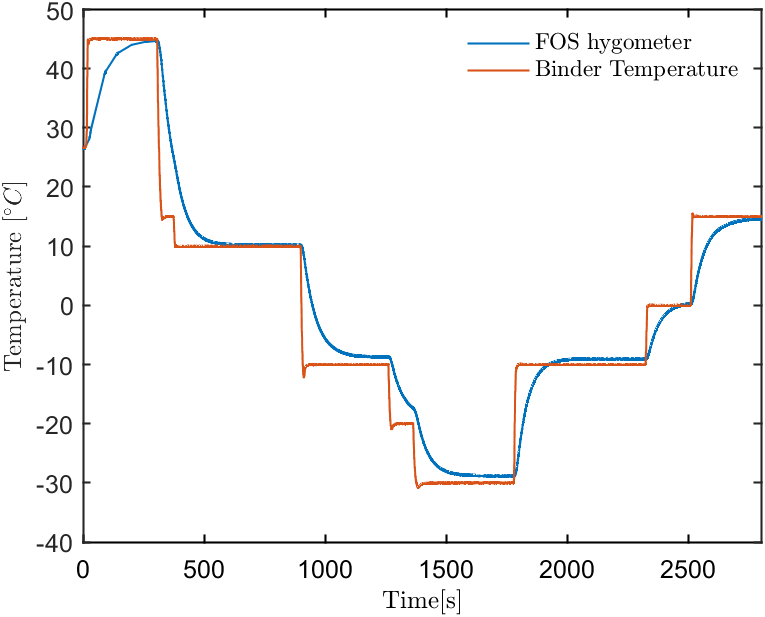
\includegraphics[width=0.47\columnwidth]{Chapter5/images/FOS_performance_T.png}
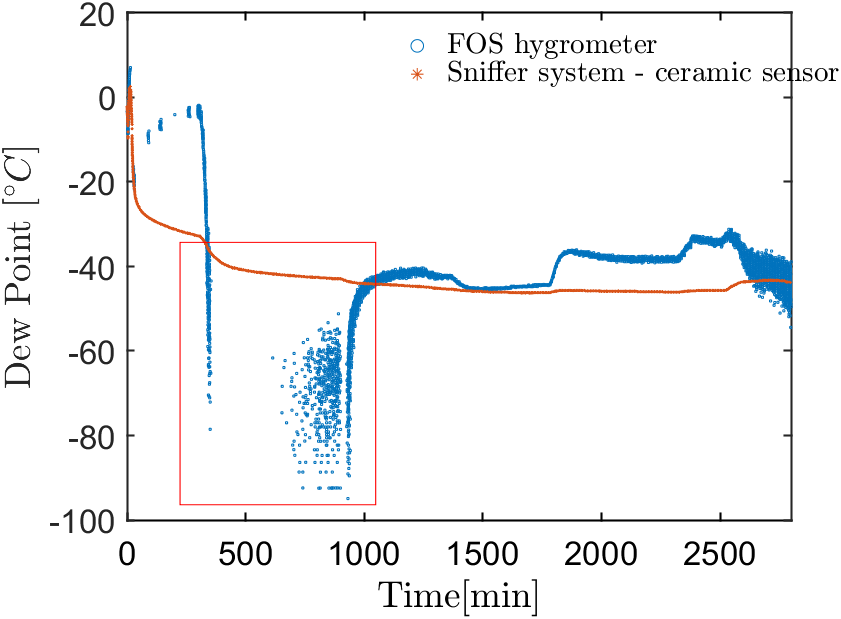
\includegraphics[width=0.49\columnwidth]{Chapter5/images/FOS_performance1.png}
\caption{A comparison of the readouts from the temperature sensors inside the Binder chamber with the \gls{FBG}-based hygrometer (left). Dew point during the changing ambient conditions per the hygrometer and the ceramic sensor.}
\label{Tfig_comparison_2}
\end{figure}

\section{Final considerations}

The characterization of the \gls{FOS} brought information on the advantages and limits of this particular technology with the use of polyimide as the sensitive material. In principle, the tested hygrometer meets the requirements set for the \gls{STS}. The distributed system will feature the sampling system, \gls{FOS}, and capacitive sensors.

An array of sensors could still be considered, but the distance between the gratings should be much larger than \SI{15}{\cm} to ensure that the sensors can be packaged in strain-free conditions. As stated in Section~\ref{fos_irrad}, the \gls{FBG} based \gls{FOS} can be considered radiation hard. According to \cite{Berruti}, the sensors can be used in radiation environments by pre-irradiating them before installation, to reduce radiation-induced cross-sensitivity. 

Moreover, the capacitive industrial sensors will be used next to the \gls{FOS}. The main purpose will be to use them during the commissioning and in order to recalibrate the \gls{FOS} if the installation will cause any additional stress on the grating.

The last technology foreseen for the distributed sensing system is the metal oxide (ceramic) moisture sensors. It is the most reliable solution that will be used also for the interlocking system. Several sampling points inside the detector enclosure will measure trace humidity and serve as a reference for the two other measurement technologies. The system should also be redundant and accurate during 10 years of operation. Therefore, a viable solution is to install a chilled mirror hygrometer in the vicinity of the sampling system readout in order to cross-check the readouts and ensure safety. 